\section{Durchführung}
\label{sec:Durchführung}

\subsection{Justierung} 
\label{sub:Justierung}


Vor Beginn des eigentlichen Versuchs müssen vorbereitende Justierungen durchgeführt werden. Beide Schwingkreise müssen 
auf die gleiche Resonanzfrequenz eingestellt werden.
Dabei wird, wie in Bild \ref{fig:bild5} dargestellt, eine variierbare Kapazität in einen der Schwingkreise geschaltet. Über ein
Oszilloskop im XY-Betrieb können Lissajous-Figuren dargestellt werden. Zuerst wird dabei eine ungefähre Ermittllung der Resonanzfrequenz vorgenommen, in dem der X-Eigang von der 
Generatorspannung getrennt wird. Durch Veränderung der Frequenz sollen die beobachtbaren Lissajous-Figuren verschwinden. Ist das der Fall, so sind Strom und Spannung in Phase. In der Praxis gestalltet sich das auf Grund von unzureichend genauen Justiermöglichkeiten relativ schwierig.
Durch eine möglichst gute Minimierung der von der Figur berandeten Fläche kann
ebenfalls in guter Näherung die Resonanzfrequenz gefunden werden. Die Schaltung wird wieder wie in Abbildung \ref{fig:bild5} aufgebaut. Daraufhin gilt es den verstellbaren Kondensator so zu justieren, sodass auch der zweite Schwingkreis auf die eben gefundene Frequenz eingestellt wird.


\begin{figure}

    \centering
    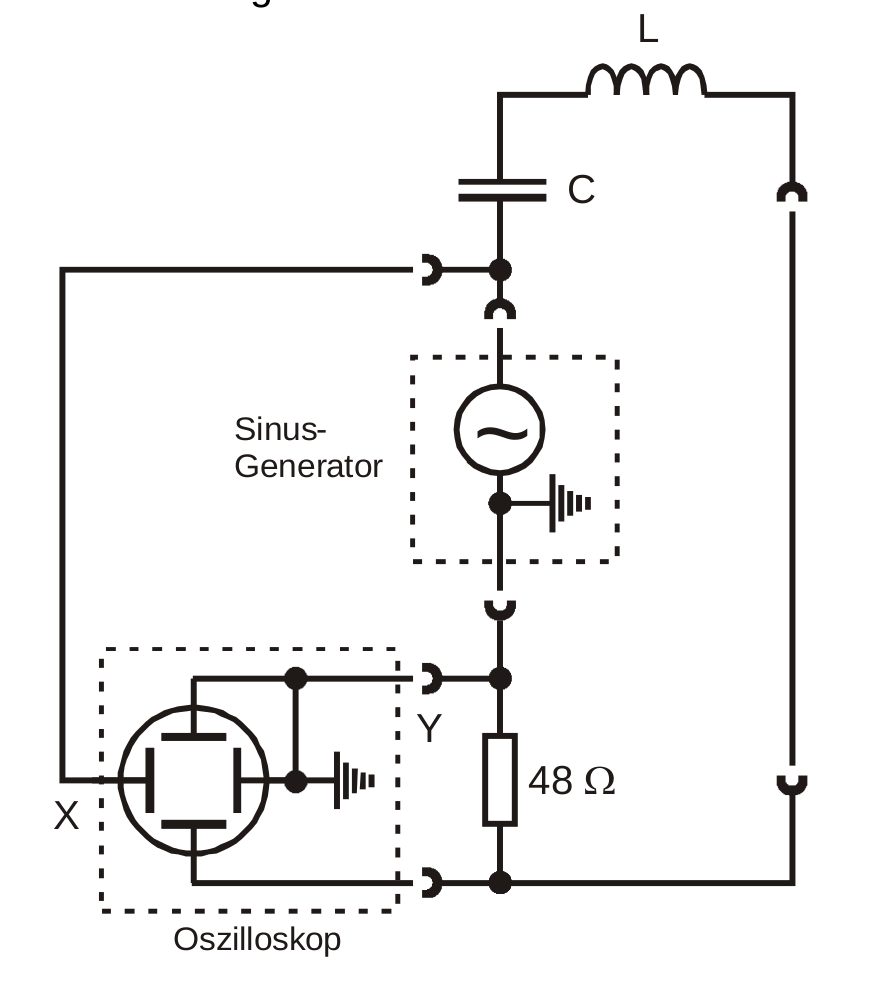
\includegraphics[height=6.0cm]{data/Bild5.png}
    \caption{Schaltbild zur Bestimmung der Resonanzfrequenz eines Schwingkreises.}
    \label{fig:bild5}
\end{figure}

\subsection{Untersuchung einer Schwebung} 
\label{sub:Untersuchung einer Schwebung}



Der Versuch soll mit Hilfe von Schwebungen den Energieaustausch zwischen den beiden Schwingkreisen darstellen.
Dafür wird die Schaltung nach Abbildung \ref{fig:bild6} aufgebaut. Es ist zu Beachtem, dass nur der linke Schwingkreis durch einen Sinusgenerator angeregt wird.
Mit Hilfe eines Oszilloskops können bei Variation des 
Kondensators $C_K$ verschiedene Schwebungen beobachtet werden. Die Kapazität wird dabei bei von $2\si{\nano\farad}$  bis $12\si{\nano\farad}$
schrittweise erhöht. Jedesmal wird anschließend das Verhältnis der beiden Frequenzen ermittelt, indem die Anzahl der Schwingungsmaxima innerhalb einer Schwebungsperiode 
gezählt werden.


\subsection{Bestimmung der Fundamentalschwingungen}
\label{sub:Bestimmung der Fundamentalschwingungen}



Der zweite Teil des Versuchs zielt auf des ermitteln der Fundamentalschwingungen ab. Die Schaltung wird, bis auf das ersetzten des Rechteckgenerators in
einen Sinusgenerator, so wie in Abbildung \ref{fig:bild6} beibehalten. Die Generatorspannung soll dabei auf den X-Eingang gegeben werden.
Durch erneute Einstellung des XY-Betriebes können wieder Lissajous-Figuren beobachtet werden. Der Kondensator $C_K$ wird wieder schrittweise verändert und jedesmal die Frequenzen ermittelt, bei 
denen die Lissajous-Figur verschwindet. 


\begin{figure}

    \centering
    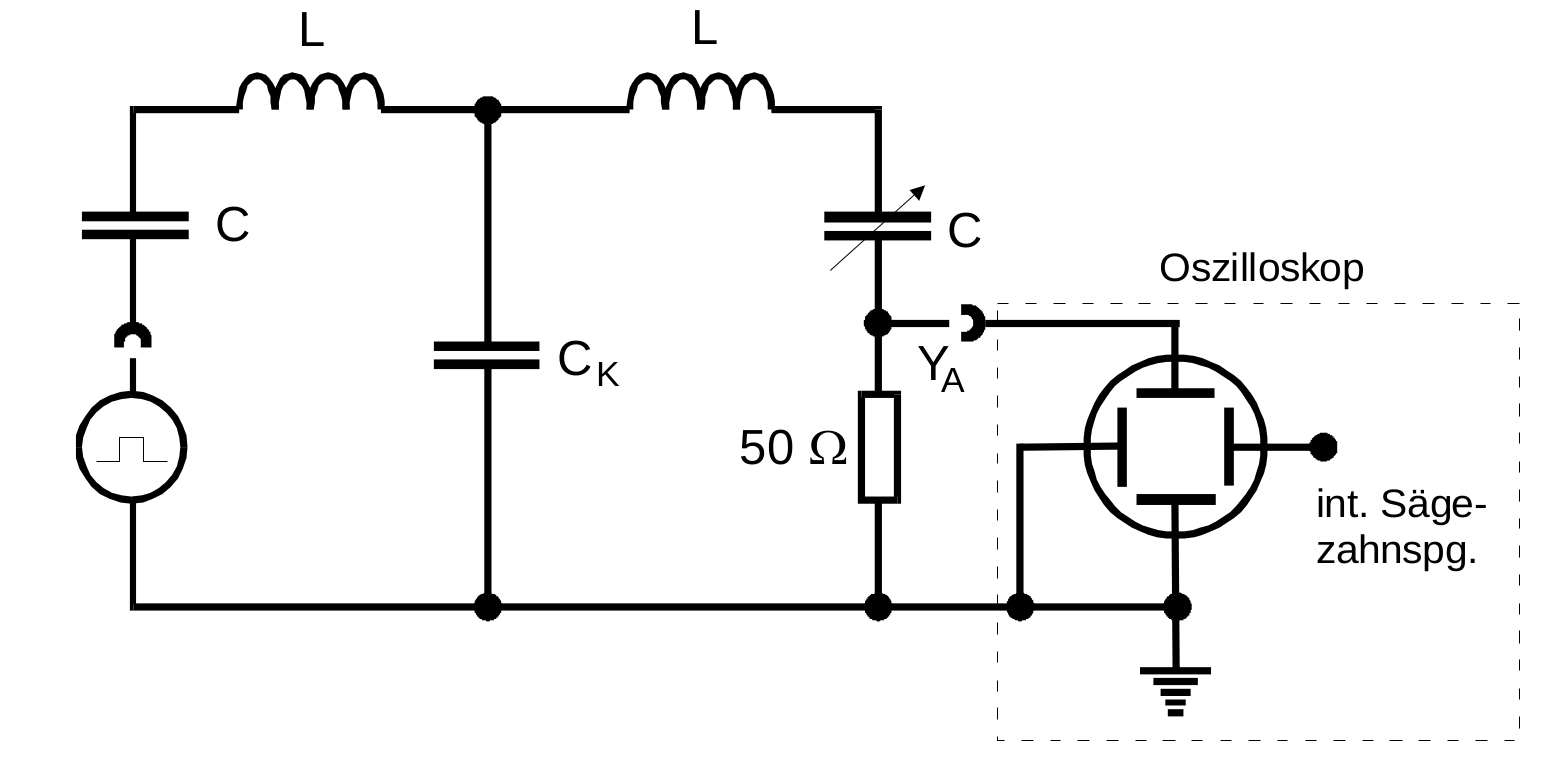
\includegraphics[height=6.0cm]{data/Bild6.png}
    \caption{Schaltbild zur Bestimmung der Fundamentalschwingungen eines gekoppelten Systems.}
    \label{fig:bild6}
\end{figure}


\subsection{Untersuchung der Ströme im gekoppelten Schwingungssystem.} 
\label{sub:Untersuchung der Ströme im gekoppelten Schwingungssystem.}

Als letztes wird der Verlauf der Ströme $I_2(\nu^+)$ und $I_2()\nu^-$ in Abhängigkeit von der Frequenz untersucht.
Dabei wird die Schaltung wie in Abbildung \ref{fig:bild8} aufgebaut.

\begin{figure}

    \centering
    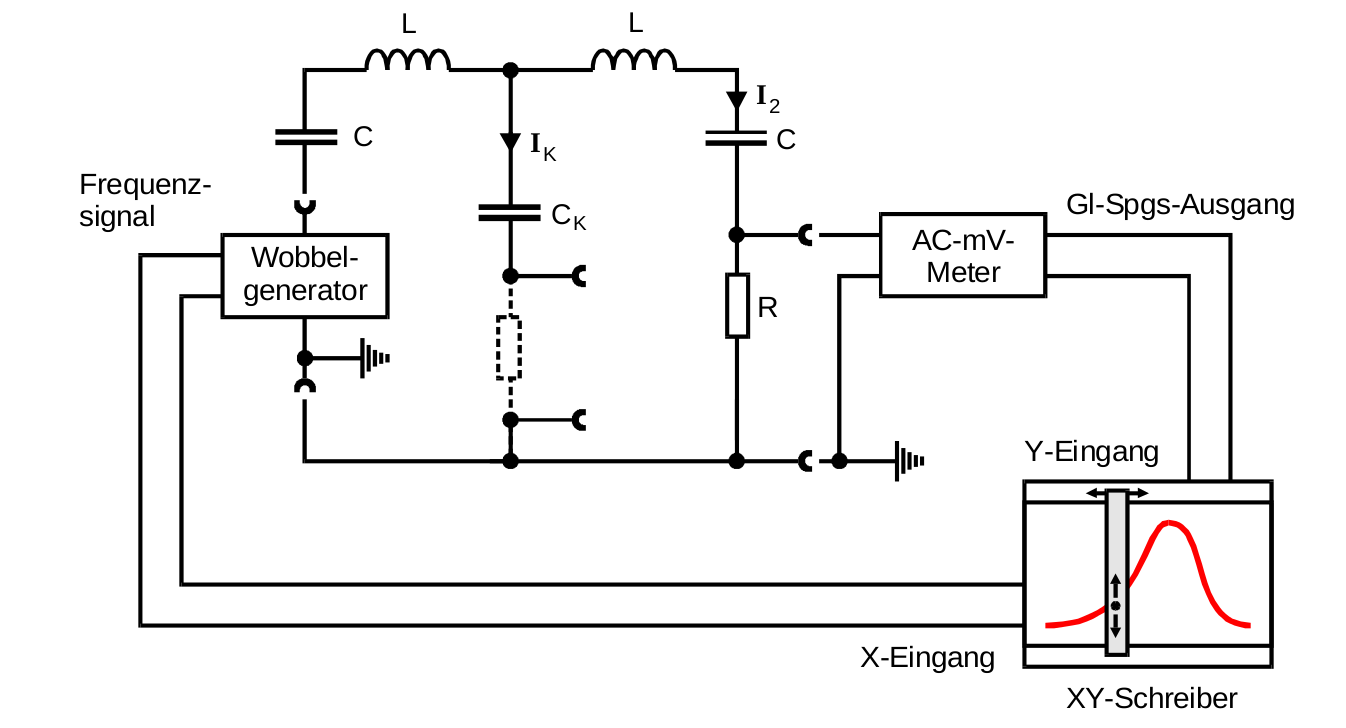
\includegraphics[height=7.0cm]{data/Bild8.png}
    \caption{Schaltbild zur Bestimmung der Fundamentalschwingungen eines gekoppelten Systems.}
    \label{fig:bild8}
\end{figure}





%Was wurde gemessen bzw. welche Größen wurden variiert?